% !TEX root = ../../thesis.tex

\documentclass[../../thesis.tex]{subfiles}
 
\begin{document}

In this chapter, we experiment our solvers and discuss the results. 

\section{Benchmark process}

We used our benchmark runner described in \autoref{section:benchmark-runner} to run our experiments.
Once all the tested solvers have finished their run, we extract the results and create a JSON file 
with the final results (objective, time, etc.). We can then create plots that make it 
easier to analyze and discuss the results. Two of those plots are \emph{timelines} and \emph{performance profiles}.

\subsection{Timelines}

A timeline is a decreasing function of the objective over time. 
They represent the average evolution of the objective of all instances over time.
However, as objectives can be 
significantly different from one instance to another, all objectives are normalized to a $[0, 1]$ range.
We call this the relative distance to the best objective. 
The normalized objective ($no$) for instance $i$ at each timestamp $t$ can 
be computed with the following formula:

\begin{equation*}
  no_i(t) = \frac{objective_i(t) - best_i}{objective_i(0) - best_i}
\end{equation*}

A value of $1$ will always be the initial solution for each solver, even though they might not be equal. A value of 
$0$ is the best solution found at the end of the search. 

For each time $t$, we take the average of all normalized objectives over all instances:


\begin{equation*}
   no(t) = \frac{\sum_{i \in \mathcal{I}} no_{i}(t)}{|\mathcal{I}|}
\end{equation*}



\begin{figure}
  \centering
  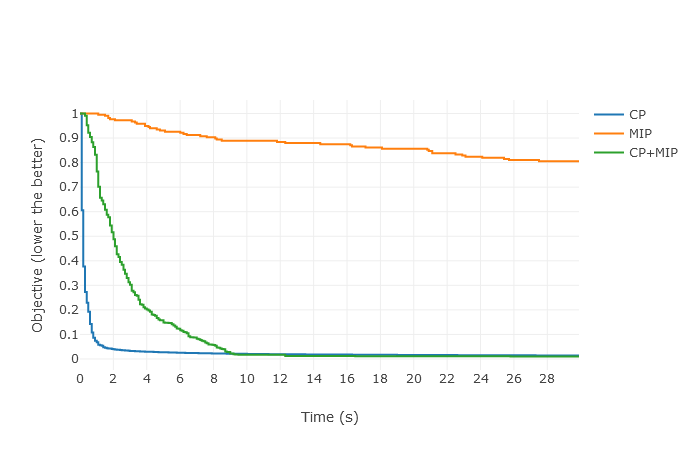
\includegraphics[scale=0.50]{experiments/solvers-oot.png}
  \caption{Example of timeline.}
  \label{timeline-example}
\end{figure}

\autoref{timeline-example} shows an example of timeline with three solvers. The $x$ axis is the time in seconds and the $y$ axis is the normalized objective 
value. In practice, we do not compute the normalized objective for every second but for every 1/10th second for more accurate results.



\subsection{Performance profiles}

A performance profile \cite{Dolan2002} is a cumulative distribution function of a performance metric (i.e. objective, time, etc.).
In our case, we are mostly interested in the objective metric after a fixed amount of time.
This is how a performance profile is computed:

For each problem $p$ and solver $s$, we define two performance metrics:

\begin{align*}
  t_{p, s} &= \text{time required to solve $p$ by solver $s$} \\
  o_{p, s} &= \text{objective of $p$ obtained by solver $s$}
\end{align*}


From these results, we can compute a performance ratio $r_{p, s}$ for a performance metric.
We use $m_{p, s}$ in the following formulas which refers to a performance metric such as $t_{p, s}$ or $o_{p, s}$.

\begin{equation}
  r_{p, s} = \frac{m_{p, s}}{min\{ m_{p, s} : s \in \mathcal{S} \}}
\end{equation}

This ratio is the comparison between the performance of a solver $s$ with the best solver for $p$.
This means that the best solver is used as baseline. However, it can be interesting to change 
the baseline to change the comparison. For this, we change the formula \cite{Cauwelaert2017AVW} to:

\begin{equation}
  r_{p, s} = \frac{m_{p, s}}{min\{ m_{p, b} : b \in \mathcal{B} \} }
\end{equation}

where $\mathcal{B} \subseteq \mathcal{S}$ is the set of baselines.
The performance profile of a solver is then given by:


\begin{equation}
  F_s(\tau) = \frac{1}{|\mathcal{P}|} \left| \left\{ p \in \mathcal{P} : r_{p, s} \leq \tau \right\} \right|
\end{equation}

with $\tau \in \mathbb{R}$ being a performance factor. In other words, $F_s(\tau)$ is the cumulative probability
of having a performance ratio within a factor $\tau$ of the best possible ratio.

\begin{figure}
  \centering
  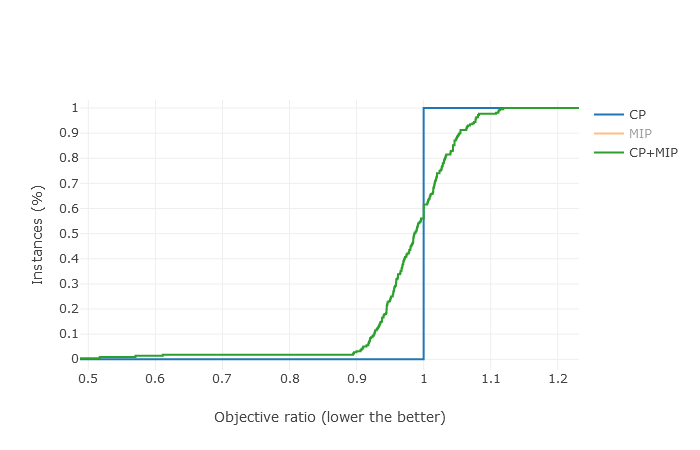
\includegraphics[scale=0.55]{experiments/cp,cp+mip-profile.png}
  \caption{Example of performance profile.}
  \label{example-profile}
\end{figure}

We can plot multiple performance profiles of different solvers, with different baselines, to compare them.
\autoref{example-profile} shows an example of performance profile with the objective as performance metric.
This profile represents the objective after a fixed amount of time 
with two solvers CP and CP+MIP with CP as 
baseline.
We can see on the $y$ axis the percentage of instances solved by the solvers and on the $x$ the objective expressed
as a ratio of the objective obtained by the baseline. We can see in this example that for around 60\% of instances,
the objective is better or equal for the CP+MIP solver with an improvement up to 10\% compared to the baseline.
In the remaining 40\% of instances, we can see that the CP+MIP solver is worse also up to around 10\%.


We can also have multiple solvers as baseline as we can see in \autoref{example-profile2} where all the solvers 
are used as baselines. In this type of profile, the objective used in the objective ratio is the best objective between all solvers.

\begin{figure}
  \centering
  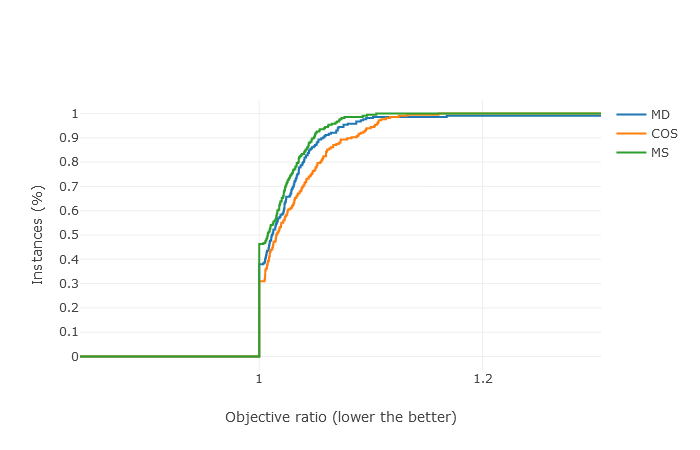
\includegraphics[scale=0.55]{experiments/cos-md-ms.png}
  \caption{Example of performance profile with all solvers as baselines.}
  \label{example-profile2}
\end{figure}


\subsection{Hardware}

All the experiments were performed on a UCLouvain server \cite{jabba} from the INGI department.

\begin{itemize}
  \item Intel(R) Xeon(R) CPU E5-2687W v3 \verb+@+ 3.10GHz 
    \begin{itemize}
      \item 20 cores available.
      \item 40 threads.
    \end{itemize}
  \item 128 Go RAM
\end{itemize}

The tests were ran mostly during the night due to the long running times and to avoid having 
perturbations from other users. However, as this machine has a high number of cores, running tests 
during the day did not impact the tests. 
The server load was still monitored from the INGI website \cite{jabba:monitoring} and the server was never overloaded.

\subsection{Benchmark Instances}

For our experiments, we generated 216 instances of different sizes. The problem sizes were based on the needs of the \vone\ company.
\autoref{instances:proportions} shows the size proportions for the 216 instances used in the experiments. $T$ represents the number of time period, $D$ the number of demands and $W$ the number of workers. The generated instances also have varying probabilities as presented in \autoref{instance:options}. These probabilities are referenced in \autoref{instances:probabilities} and follow a uniform distribution where $P_{\mu} = \frac{P_{min} + P_{max}}{2}$.


\begin{table}[H]
  \caption{Proportions of instance sizes for 216 instances}
  \label{instances:proportions}
  \centering
  \begin{tabular}[t]{|c|c|c |c|c|}
    \hline
    \multicolumn{3}{|c|}{Size} & \multicolumn{2}{|c|}{Prop.} \\
    \hline 
    $T$ & $D$ & $W$ & $n$ & $\%$ \\
    \hline 
    \multirow{9}{*}{5} & \multirow{3}{*}{30} & 150 & 8 & 3.7 \\ 
    \cline{3-5}
     &  & 225 & 8 & 3.7 \\ 
     \cline{3-5}
     &  & 300 & 8 & 3.7 \\ 
     \cline{2-5}
     & \multirow{3}{*}{40} & 150 & 8 & 3.7 \\ 
     \cline{3-5}
     &  & 225 & 8 & 3.7 \\ 
     \cline{3-5}
     &  & 300 & 8 & 3.7 \\ 
     \cline{2-5}
     & \multirow{3}{*}{50} & 150 & 8 & 3.7 \\ 
     \cline{3-5}
     &  & 225 & 8 & 3.7 \\ 
     \cline{3-5}
     &  & 300 & 8 & 3.7 \\ 
    \hline
  \end{tabular}
  \hfill
  \begin{tabular}[t]{|c|c|c |c|c|}
    \hline
    \multicolumn{3}{|c|}{Size} & \multicolumn{2}{|c|}{Prop.} \\
    \hline 
    $T$ & $D$ & $W$ & $n$ & $\%$ \\
    \hline 
    \multirow{9}{*}{10} & \multirow{3}{*}{30} & 150 & 8 & 3.7 \\ 
    \cline{3-5}
     &  & 225 & 8 & 3.7 \\ 
     \cline{3-5}
     &  & 300 & 8 & 3.7 \\ 
     \cline{2-5}
     & \multirow{3}{*}{40} & 150 & 8 & 3.7 \\ 
     \cline{3-5}
     &  & 225 & 8 & 3.7 \\ 
     \cline{3-5}
     &  & 300 & 8 & 3.7 \\ 
     \cline{2-5}
     & \multirow{3}{*}{50} & 150 & 8 & 3.7 \\ 
     \cline{3-5}
     &  & 225 & 8 & 3.7 \\ 
     \cline{3-5}
     &  & 300 & 8 & 3.7 \\ 
    \hline
  \end{tabular}
  \hfill
  \begin{tabular}[t]{|c|c|c |c|c|}
    \hline
    \multicolumn{3}{|c|}{Size} & \multicolumn{2}{|c|}{Prop.} \\
    \hline 
    $T$ & $D$ & $W$ & $n$ & $\%$ \\
    \hline 
    \multirow{9}{*}{15} & \multirow{3}{*}{30} & 150 & 8 & 3.7 \\ 
    \cline{3-5}
     &  & 225 & 8 & 3.7 \\ 
     \cline{3-5}
     &  & 300 & 8 & 3.7 \\ 
     \cline{2-5}
     & \multirow{3}{*}{40} & 150 & 8 & 3.7 \\ 
     \cline{3-5}
     &  & 225 & 8 & 3.7 \\ 
     \cline{3-5}
     &  & 300 & 8 & 3.7 \\ 
     \cline{2-5}
     & \multirow{3}{*}{50} & 150 & 8 & 3.7 \\ 
     \cline{3-5}
     &  & 225 & 8 & 3.7 \\ 
     \cline{3-5}
     &  & 300 & 8 & 3.7 \\ 
    \hline
  \end{tabular}
\end{table}


\begin{table}[H]
  \caption{Probability range for generated instances}
  \label{instances:probabilities}
  \centering
  \begin{tabular}[t]{|l r r|}
    \hline 
    $P_{name}$ & $P_{min}$ & $P_{max}$ \\
    \hline
    assignSkill & 0.1 & 0.3 \\
    assignWorkerSkill & 0.1 & 0.3 \\
    assignPeriod & 0.4 & 0.8 \\
    assignLocation & 0.3 & 0.7 \\
    assignMachines & 0.1 & 0.5 \\
    takeMachine & 0.1 & 0.3 \\
    assignWorkingRequirements & 0.1 & 0.3 \\
    assignWWI & 0 & 0.1 \\
    assignWCI & 0 & 0.1 \\
    \hline
  \end{tabular}
\end{table}

\section{Constraint Programming}

\subsection{Comparison between heuristics}

We talked in \autoref{section:cpmodel} about our custom heuristic called Most Available Heuristic.
We now compare the performance of this heuristic with standard heuristic like the Max Value heuristic.
We also compare the variable heuristics used in addition to our aforementioned heuristic.

\subsubsection{Value heuristic}

We compare multiple value heuristics:

\begin{itemize}
  \item The Max Value heuristic. This heuristic simply takes the maximum value in the domain of the variable. We 
  take the maximum instead of the minimum because of the sentinel value being equal to -1 in every domain. 
  \item The Most Available heuristic discussed in \autoref{section:cpmodel}.
  \item The Dynamic Most Available heuristic also discussed in \autoref{section:cpmodel}.
\end{itemize}

We first start by comparing the Max Value and the static Most Available heuristics together.
\autoref{experiments:heuristic1} shows the objective ratio between the implemented custom Most Available heuristic and a standard 
Max Value heuristic after the first solution.
The two heuristics were tested on 72 instances of various sizes from small to big instances.
The performance profile shows a clear gain of about $2$ to $3.4$ for our custom heuristic.

Heuristics like Max Value are ones of the simpler heuristics to implement but often offer bad performance due to 
the lack of knowledge of the problem.


\begin{figure}
  \centering
  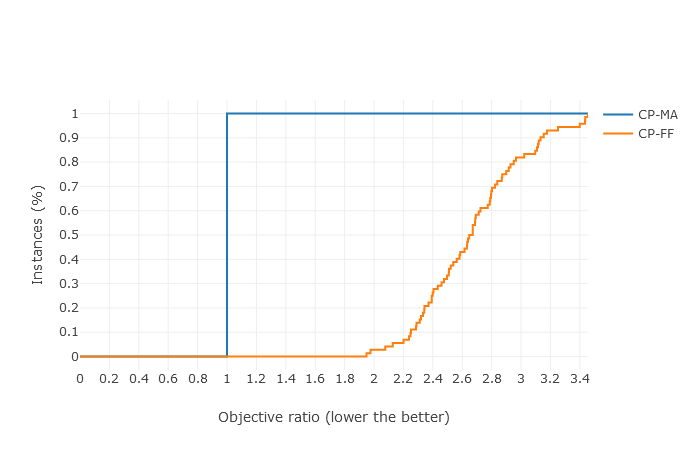
\includegraphics[scale=0.55]{experiments/heuristic.png}
  \caption{Most Available and First Fail heuristics [72 instances/first solution].}
  \label{experiments:heuristic1}
\end{figure}

\paragraph{}

We now compare our static and dynamic Most Available heuristics together.
\autoref{experiments:heuristic2} shows the performance profile of the dynamic and static \texttt{mostavailable} heuristics.
We can see that the dynamic version of the heuristic outperforms the static one in every instances.
Even though the dynamic version need to process more during the search, we can see that the time lost 
by this processing is gained back during the search.

\paragraph{}

As our dynamic value heuristic outperforms other tested value heuristics, we will assume for the rest of this chapter 
that the value heuristic for the Constraint Programming solver is the dynamic \texttt{mostavailable}.


\begin{figure}
  \centering
  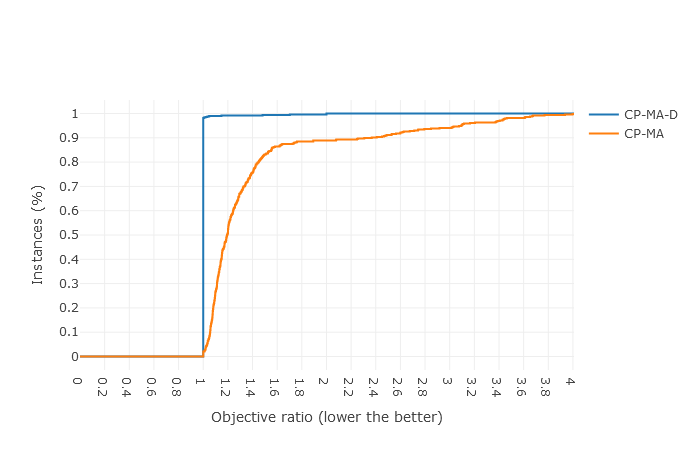
\includegraphics[scale=0.55]{experiments/static-dynamic-heuristic.png}
  \caption{Most Available: static and dynamic [486 instances/15s].}
  \label{experiments:heuristic2}
\end{figure}


\subsubsection{Variable heuristic}

In addition to our \texttt{mostavailable} heuristic, we use a variation of the \texttt{maxdegree} heuristic. 
This heuristic is a first-fail variable heuristic that selects the most constrained unbound variable. However,
as stated in our model in \autoref{section:cpmodel}, skills are not represented with constraints but instead values 
are removed from the domain at initialization. To express skills as part of the max degree, we simply add the number of 
skills required by a variable to the degree of that variable.


We compare multiple variable heuristics:

\begin{itemize}
  \item Custom Max Degree (MD) heuristic
  \item Min Size (MS) heuristic. The Min Size heuristic simply selects the variable with minimum domain size.
  \item Conflict Ordering Search (COS) heuristic
\end{itemize}


Conflict Ordering Search (COS) \cite{Gay:COS} is a variable ordering heuristic that 
reorders variables based on the number of conflicts that happen during the search.
It is a variant to the Last Conflict heuristic that selects the variable which caused the last conflict first.
COS was shown to be the most performant on scheduling problems. We will now see how it performs in our problem.

\autoref{experiments:heuristics:3} shows a performance profile for the objective after 30s for each solver.
We can see that the three heuristics are very close of each other. However, the Min Size heuristic performs slightly better the Max Degree heuristic with the 
COS heuristic coming last.


\begin{figure}
  \centering
  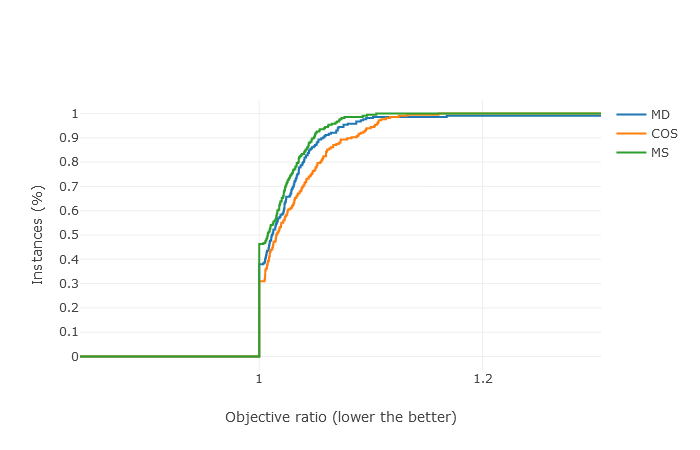
\includegraphics[scale=0.55]{experiments/cos-md-ms.png}
  \caption{COS, Max Degree and Min Size heuristics [216 instances/30s].}
  \label{experiments:heuristics:3}
\end{figure}

The three heuristics perform well and changing between these heuristics will not show a significant improvement.

TODO: Solution/time

\subsection{Comparison between searches}


As stated in \autoref{chapter:sota} and \autoref{section:cpmodel}, LNS is used to expand the exploration
of the search tree. We now compare our solver with the use of LNS and without. We also compare multiple 
relaxations method.


\autoref{experiments:lns} shows the performance profile for the final objective after 30s of search 
between a standard search and LNS. As expected, we can see that LNS outperforms the standard search 
in every instances. \autoref{experiments:lns-oot} shows that the standard search quickly get stuck
while the LNS manages to find better solutions quickly after relaxing the initial solution.


\begin{figure}
  \centering
  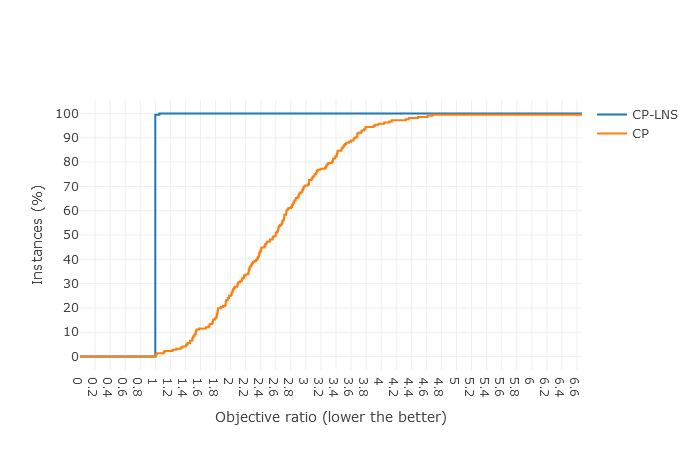
\includegraphics[scale=0.55]{experiments/lns-profile.png}
  \caption{CP with and without Large Neighborhood Search [216 instances/30s].}
  \label{experiments:lns}
\end{figure}

\begin{figure}
  \centering
  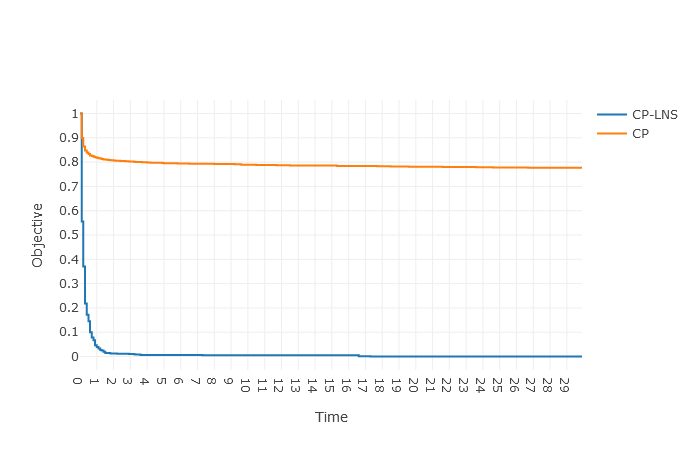
\includegraphics[scale=0.55]{experiments/lns-oot.png}
  \caption{CP with and without Large Neighborhood Search [216 instances/3s].}
  \label{experiments:lns-oot}
\end{figure}



We also experimented with multiple relaxations in the LNS framework. We compared:

\begin{itemize}
  \item Random relaxation with 40\% relaxation (CP-Random-40)
  \item Random relaxation with 50\% relaxation (CP-Random-50)
  \item Random relaxation with 60\% relaxation (CP-Random-60)
  \item Random relaxation with 70\% relaxation (CP-Random-70)
  \item Random relaxation with 80\% relaxation (CP-Random-80)
  \item Propagation based relaxation (CP-Prop)
\end{itemize}


\autoref{experiments:relax-profile} shows the performance profile for the objective after 30s with 
CP-Prop as baseline.
We can observe that overall, CP-Random-40 finds a better objective in 80\% of instances. However,
no relaxation finds a better solution in every instances. 


\autoref{experiments:relax-profile} shows that in average CP-Random-40 is the fastest to find a solution close 
to the best one with CP-Random-50 close behind.

\begin{figure}
  \centering
  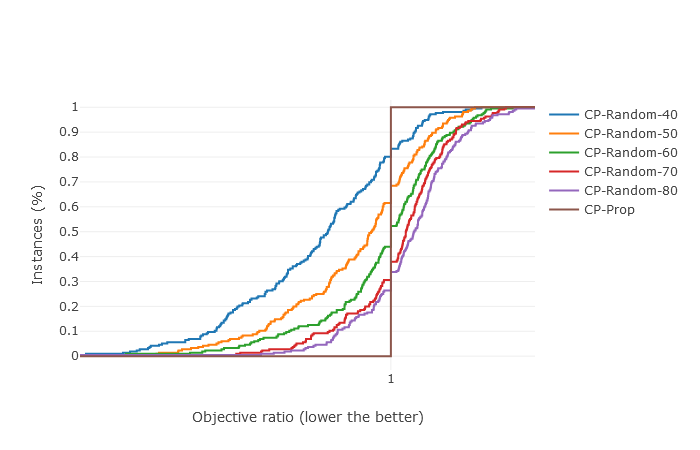
\includegraphics[scale=0.55]{experiments/relax-profile.png}
  \caption{Comparison between multiple relaxations [216 instances/30s].}
  \label{experiments:relax-profile}
\end{figure}

\begin{figure}
  \centering
  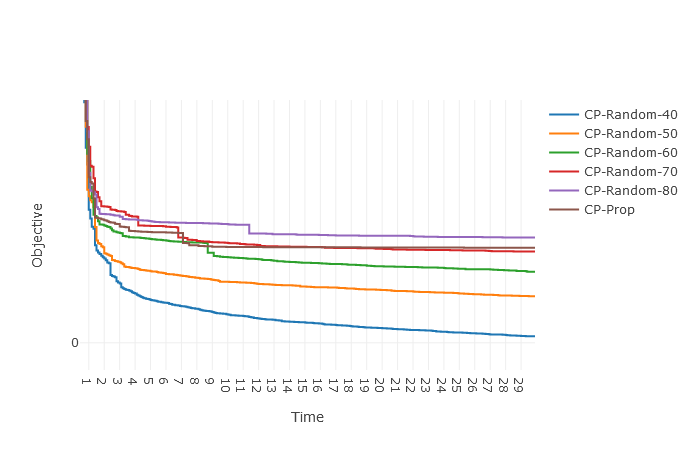
\includegraphics[scale=0.55]{experiments/relax-oot.png}
  \caption{Comparison between multiple relaxations [216 instances/30s].}
  \label{experiments:relax-oot}
\end{figure}




\section{Comparison between solvers}

We now start by comparing different solvers together. We experiment with three solvers: 

\begin{itemize}
  \item The Constraint Programming (CP) solver.
  \item The Mixed Integer Programming (MIP) solver.
  \item A combination of CP and MIP (CP+MIP) solvers. We take an initial solution from the CP solver 
  and give it to the MIP solver as start solution. 
\end{itemize}



\autoref{experiments:solvers:profile} 
shows a performance profile with the CP solver as baseline. We can clearly see that 
the MIP solver underperforms for most instance. However, it outperforms the CP solver for approximately
20\% of instances. [TODO insert figure] shows that MIP has trouble finding good objectives when the 
problem grows. Too many variables (\char`\~ 1,000,000 binary variables for the biggest instances) make it hard for a MIP model to perform well.

We can also observe from that performance profile, and in \autoref{experiments:solvers:profile2}, that 
the CP+MIP solver gives the best objective in 60\% of instances. For the remaining instances, the objective is only worse by maximum 10\%. 
The MIP solver performs a lot better when given an initial solution to work with.

\begin{figure}
  \centering
  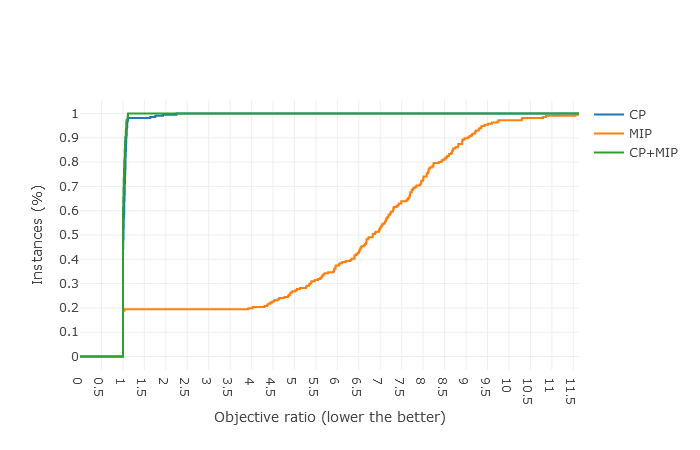
\includegraphics[scale=0.55]{experiments/solvers-profile.png}
  \caption{CP, MIP and CP+MIP solvers [216 instances/30s].}
  \label{experiments:solvers:profile}
\end{figure}

\begin{figure}
  \centering
  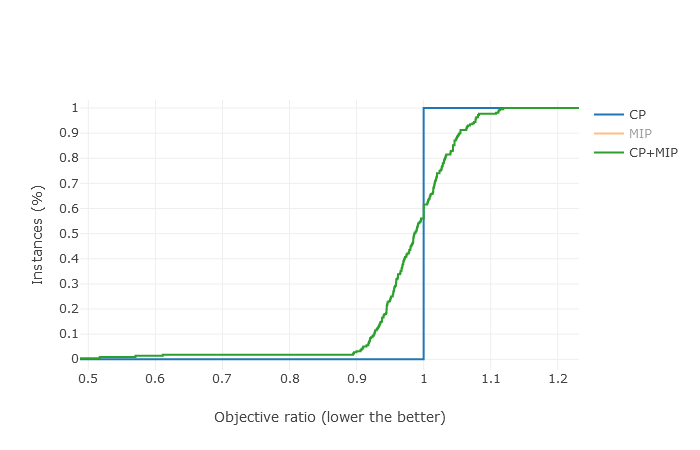
\includegraphics[scale=0.55]{experiments/cp,cp+mip-profile.png}
  \caption{CP, MIP and CP+MIP solvers [216 instances/30s].}
  \label{experiments:solvers:profile2}
\end{figure}



\autoref{experiments:solvers:oot} gives the objective per time for the three solvers. As expected from our previous results, the MIP solver does not 
give a good solution after the elapsed time. However, while the CP+MIP solver is slightly better in terms of final objective, it takes in average 10 seconds 
to reach such objective while the CP solver only takes 1 second to reach an objective really close to the final one.

% Those 20\% match with the small instances proportions in \autoref{instances:proportions}


\begin{figure}
  \centering
  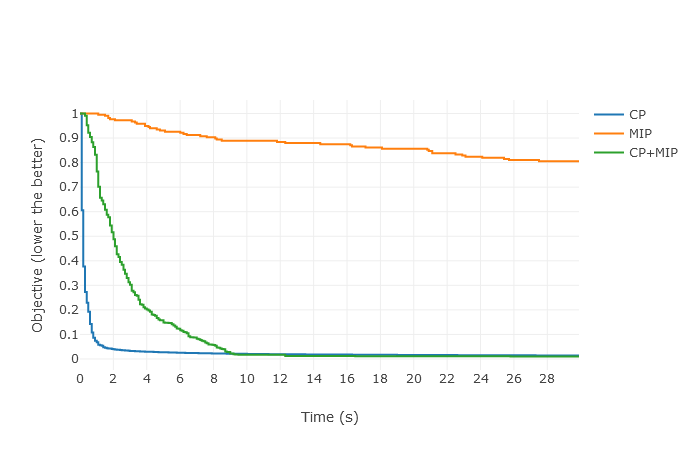
\includegraphics[scale=0.55]{experiments/solvers-oot.png}
  \caption{CP, MIP and CP+MIP solvers [216 instances/30s].}
  \label{experiments:solvers:oot}
\end{figure}


\begin{figure}
  \centering
  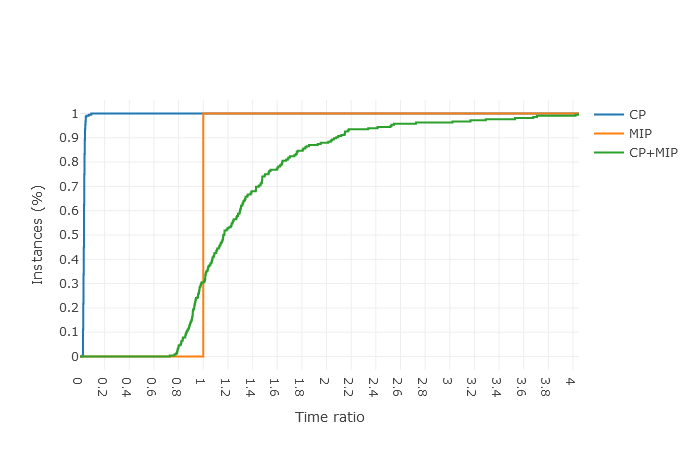
\includegraphics[scale=0.55]{experiments/time-first-sol.png}
  \caption{Time on first solution [216 instances/First solution].}
  \label{experiments:first-sol-time}
\end{figure}


\begin{figure}
  \centering
  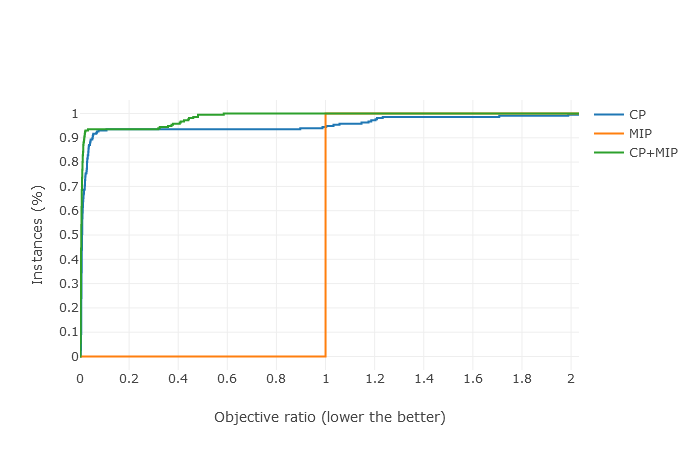
\includegraphics[scale=0.55]{experiments/obj-first-sol.png}
  \caption{Objective on first solution [216 instances/First solution].}
  \label{experiments:first-sol-obj}
\end{figure}




\end{document}

